\documentclass[conference]{IEEEtran}
\IEEEoverridecommandlockouts
% The preceding line is only needed to identify funding in the first footnote. If that is unneeded, please comment it out.
\usepackage{cite}
\usepackage{amsmath,amssymb,amsfonts}
\usepackage{algorithmic}
\usepackage{graphicx}
\usepackage{textcomp}
\usepackage{xcolor}
\def\BibTeX{{\rm B\kern-.05em{\sc i\kern-.025em b}\kern-.08em
    T\kern-.1667em\lower.7ex\hbox{E}\kern-.125emX}}
\begin{document}

\title{Clustering Analysis of Popular Music Genres Over the 2010s}

\author{\IEEEauthorblockN{Angel Sarmiento}
\IEEEauthorblockA{\textit{Department of Data Science and Business Analytics} \\
\textit{Florida Polytechnic University}\\
Lakeland, Florida, United States \\
asarmiento@floridapoly.edu}
}

\maketitle

\begin{abstract}
We demonstrate the relationships between multiple genres of music through track and album analysis using Spotify metrics. The Spotify metrics and data are wrangled using the Spotify Web API in a wrapper in R called  \textit{spotifyr}.  Regression is used to view the relationship between the \textit{emotional} metrics and other metrics. Hierarchical clustering is employed to generate insights in unseen comparisons for different albums for possible use in recommendation algorithm construction. 
\end{abstract}

\begin{IEEEkeywords}
valence, Hierarchical Clustering, regression, Spotify
\end{IEEEkeywords}

\section{Introduction}
There has been plenty of recommendation algorithms in music streaming services developed to give listeners a constant stream of music to stay interacted with the platform. Typically this involves a supervised learning algorithm. For this investigation, unsupervised learning in the form of hierarchical clustering to group albums and songs into distinct groups that can then be referenced as being related. 

This work is mainly to explore the kinds of groupings a hierarchical clustering algorithm might make for music that, at the surface level, would seemingly be dissimilar.

Another facet of this work is to see which metrics affect other metrics in the music and determine how these metrics change over the period of the 2010's. The majority of the data is pulled from the Spotify API and referenced from \textit{Pitchfork's} top 200 albums of the decade. These are meant to be a sample of the most popular music of the decade. 

\section{Background}

\subsection{Spotify and the  Web API}

Spotify is a music streaming service that caters to music audiences with recommendations, curated playlists, and user statistics. It is a very popular streaming service often touted for their superb recommendations and UI design. Their recommendation algorithm is a secret but they publish an API that includes a number of track-based metrics that are created by them. 

These metrics include: valence, speechiness, acousticness, instrumentalness, liveness, energy, and danceability. As well as more music theory based metrics like time signature, key,  mode, and tempo. Valence is a measure from 0.0 to 1.0 for the level of joyfulness exhibited by a track. Speechiness is a measure from 0.0 to 1.0 of the level of spoken word detected in a track. Acousticness represents the confidence of a track being acoustic (non-electronic). Danceability is a metric for how suitable a track is for dancing. Danceability is a combination of musical elements like tempo, beat strength, rhythm, and overall regularity \cite{b4}. Energy is a perceptual measure of intensity and activity. This means genres like heavy metal will mostly be near 1.0 whilst classical music will be closer to 0.0 \cite{b4}. Instrumentalness is a measure of the lack of vocals in a track. The last metric was Popularity, the amount of streams in a time period that Spotify receives on a specific track.

This API was accessed through a community-created wrapper in R named \textit{spotifyr}.

\subsection{Regression Analysis}

Normal regression analysis was conducted with the objective of inferring the correlational relationships between the different metrics and valence. Setting valence as the response variable allowed for variable importance to further bolster the assertions made by the EDA. This also includes the usage of correlation plots to map out the possibility of multicollinearity among the pairwise groupings of each of the parameters. 

\subsection{Locally Estimated Scatter Plot Smoothing}

Locally estimated scatter plot smoothing (LOESS) is a technique in which a regression line is fitted to data that is heavily location biased due to larger density of the surrounding data. This gives the best line of fit (often overfitting) to the data while minimizing error. The locality weighting is determined by a weight function which is commonly the so-called tri-cube weight function.

\begin{equation}
w(x) = (1 - |d|^3)^3 
\end{equation}

Where $d$ is the distance of a given data point from the point being estimated on the curve, scaled to be a value between 0 to 1 \cite{b8}.

The algorithm can use any degree of polynomial, so high degrees can result in too much variance while too low degree polynomials may not accurately interpolate fluctuations in the data \cite{b7}. 

\subsection{Hierarchical Clustering}

For Hierarchical Clustering, the method employed here will be agglomerative clustering with complete-linkage. At each combination step, the two clusters with the furthest members that are closest to each other are combined. This is done until one large cluster remains \cite{b2}. This is different from normal clustering in that k-means is not used. The formula used is shown as below:
\begin{equation}
d(G_i, G_j) = \max_{x^r \epsilon G_i , x^s \epsilon G_j} d(X^r, X^s)
\end{equation}

Where:
\begin{itemize}
\item $d(X^r, X^x)$ is the distance between instance $X^r$ and $X^s$ depending on a distance measure.
\item $G_i$: Cluster i
\item $X_i$: Instance i
\end{itemize}


\section{Methods}

\subsection{EDA and Trends}

The main objective of this work is to develop a reliable way of hierarchically clustering albums that would potentially be useful in future development of recommendation algorithms. In order to understand what might come out of the hierarchical clustering as a likely outcome, some exploratory data analysis (EDA) was done. 

The EDA involved Ridge plots, Time series plots, and correlation plots. The ridge plots are used to display a distribution of a metric across an album. The time series plots are used to display the upward or downward trend of a metric over time. 


\subsection{Data Transformation}

For Album-wise comparisons, each of the parameters were averaged across the album.  All of the variables are continuous nominal data so there were no categorical data included. The spotify data separates albums and songs so a left-join was applied to create the final dataset for use. The genre tags were obtained from the lastfmR package which pulls from the `Last.fm` API. More data wrangling was done to clean and pre-process the data for the Hierarchical Clustering and for certain plots. 


\section{Results and Discussion}

The data were pulled from the Spotify API and combined together using a playlist published by Pitchfork themselves. This playlist includes 196 of the previously mentioned 200 best songs from the best albums of the 2010s. Combined with Spotify's own popularity metric, this was then subsetted to select the most popular albums across the list of 200 and ranked as such. These will be hereby referred to as the "best" albums of the decade. 

\subsection{How Joyful are the Most Popular Albums?}

Valence, Spotify's metric for joyfulness, was the first metric analyzed using a comparative EDA across the albums. Implementing a ridge plot in Figure~\ref{fig:most-joyful}, it is possible to see where albums lie in comparison to one another level of joy. 

\begin{figure}[htbp]
\centerline{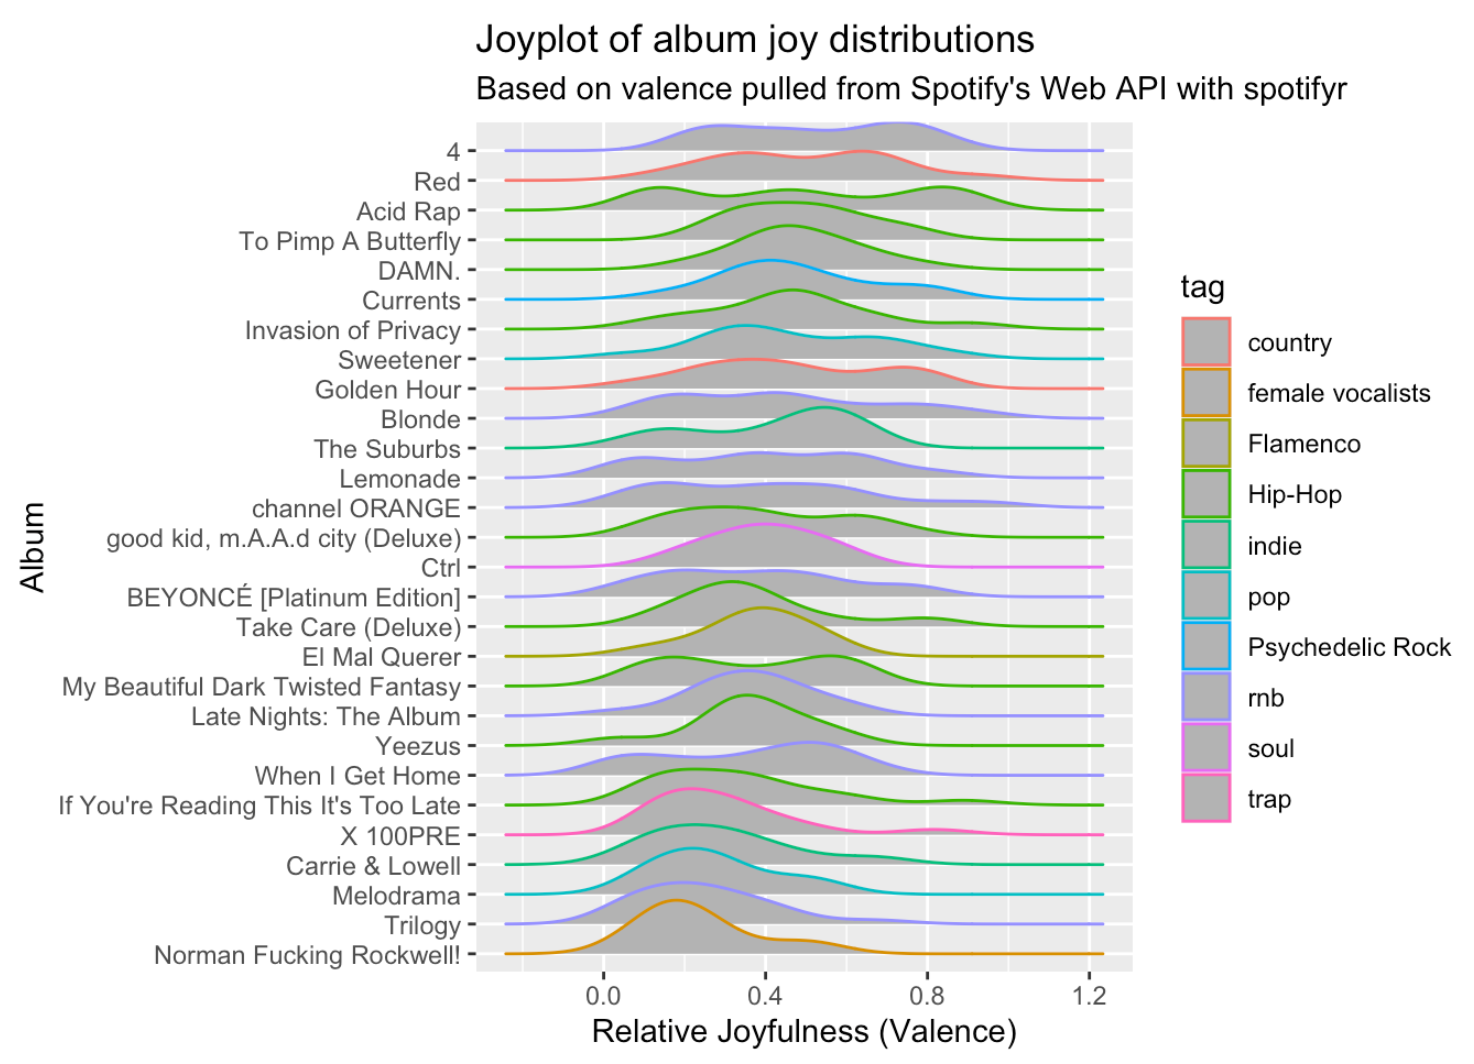
\includegraphics[width=\columnwidth]{spotify-images/most-joyful.png}}
\caption{Ridge plot of Songs over the last decade.}
\label{fig:most-joyful}
\end{figure}

This plot allows us to visualize not only where the genres of the most popular albums place in terms of joyfulness, but also allows us to visualize the general feeling of joy across the album. Figure ~\ref{fig:most-joyful} shows that hip hop albums are generally happier than genres like indie and pop. This is surprising as pop is generally consider to be a happier form of music, especially considering conventional opinions of Hip hop and its sub-genres. 

One of the top spots is held by a country album which is actually surpassed by an RnB album. RnB stands for "Rhythm and Blues" and is generally a much moodier genre that relies on the emotional weight of songwriting choices \cite{b9}. 

One thing to also note here is that the lowest album with "female vocalist" as the tag is on the opposite spectrum when compared to hip hop. The tag "female vocalist" is not a tag but is a result of too many tags for a selected artists music. The album is in fact alternative/indie.

\subsection{Is Vocal-heavy Music Happier?}

Since hip hop albums seemed to take a higher spot on the album list ranked by joy and hip-hop is a more vocal-heavy genre \cite{b8}, is there a relation between how vocal-heavy an album is and how sad it is?
Figure ~\ref{fig:sad-words} shows the related ridge ("joy") plot for this, where descending the graph is descending in the vocality of albums. 

\begin{figure}[htbp]
\centerline{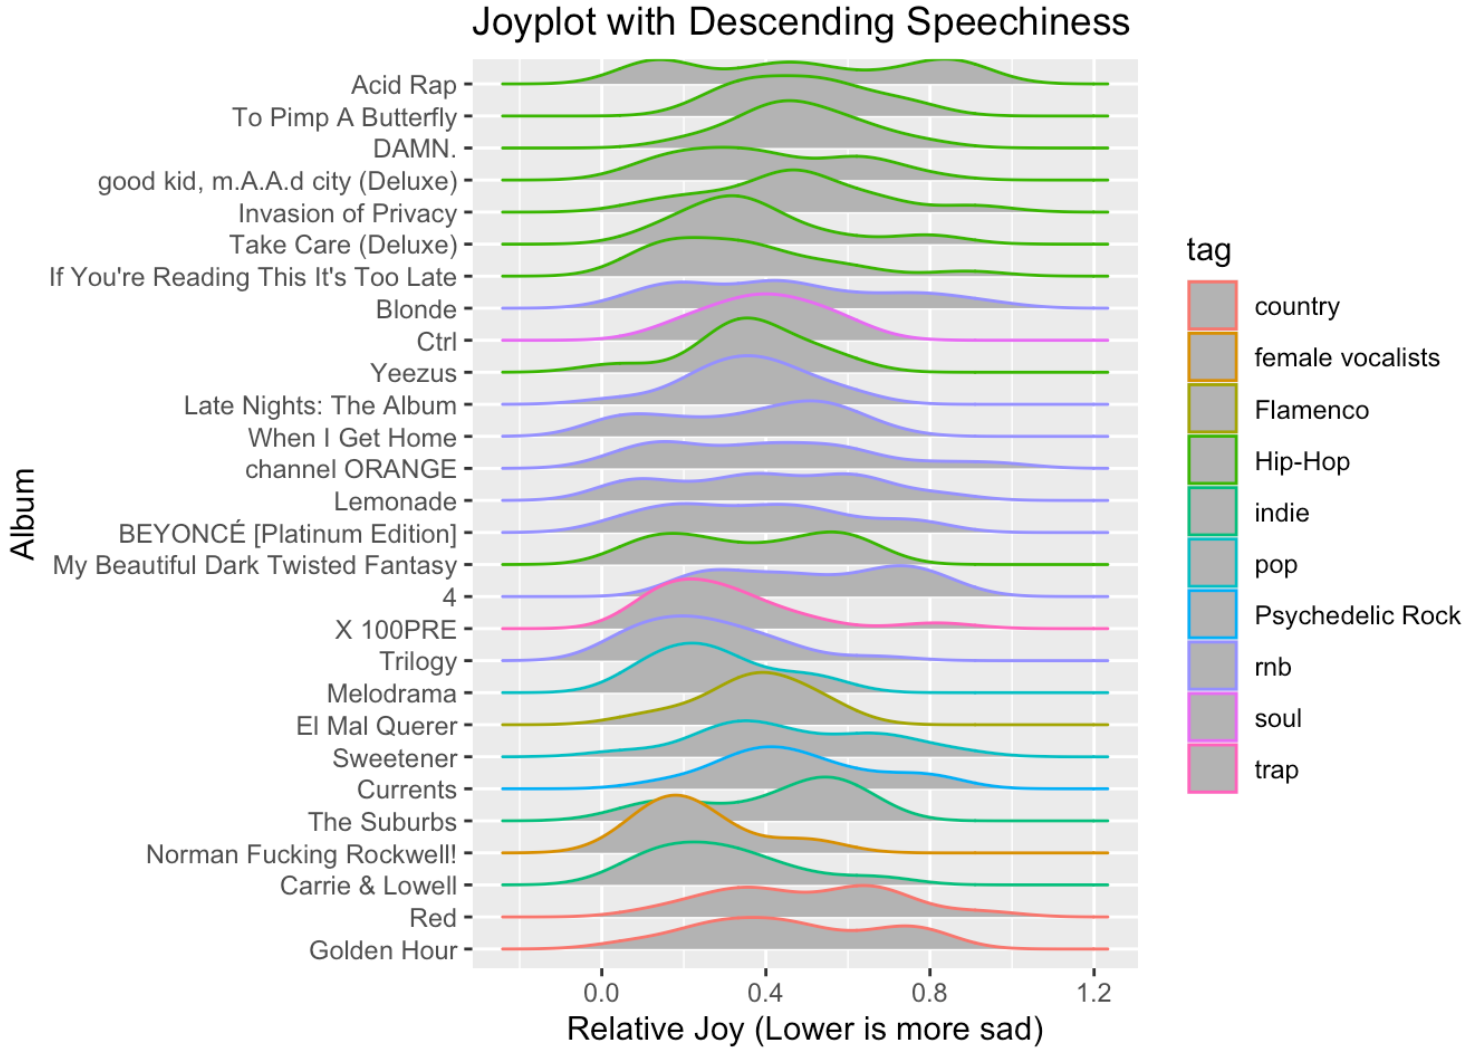
\includegraphics[width=\columnwidth]{spotify-images/sad-words.png}}
\caption{Ridge plot of Songs over the last decade.}
\label{fig:sad-words}
\end{figure}

There does not seem to be a strong correlation between vocalness and joyfulness, but there is some. With Fig. ~\ref{fig:sad-words} however, we can see that rnb is a fairly vocal heavy and a bit more sad than hip hop generally is. 

From these plots, we might expect a clustering algorithm to link genres like rnb and hip-hop together. There are most likely more underlying relations that can be made from this data. Maybe there is some correlation between the other variables and valence (joyfulness) that have not been addressed? 

\subsection{Collinearity and Regression}

What are the relationships between the different variables? There are most likely some significance in using the other variables to estimate the value of valence. For this, we will use regression analysis to see what variables are significant. 

Fig.~\ref{fig:corrplot} shows correlation plot between the variables to map what might be an underlying pairwise interaction to be included in a regression analysis. This also helps to identify any multicollinearity that may be present in the data. 

\begin{figure}[htbp]
\centerline{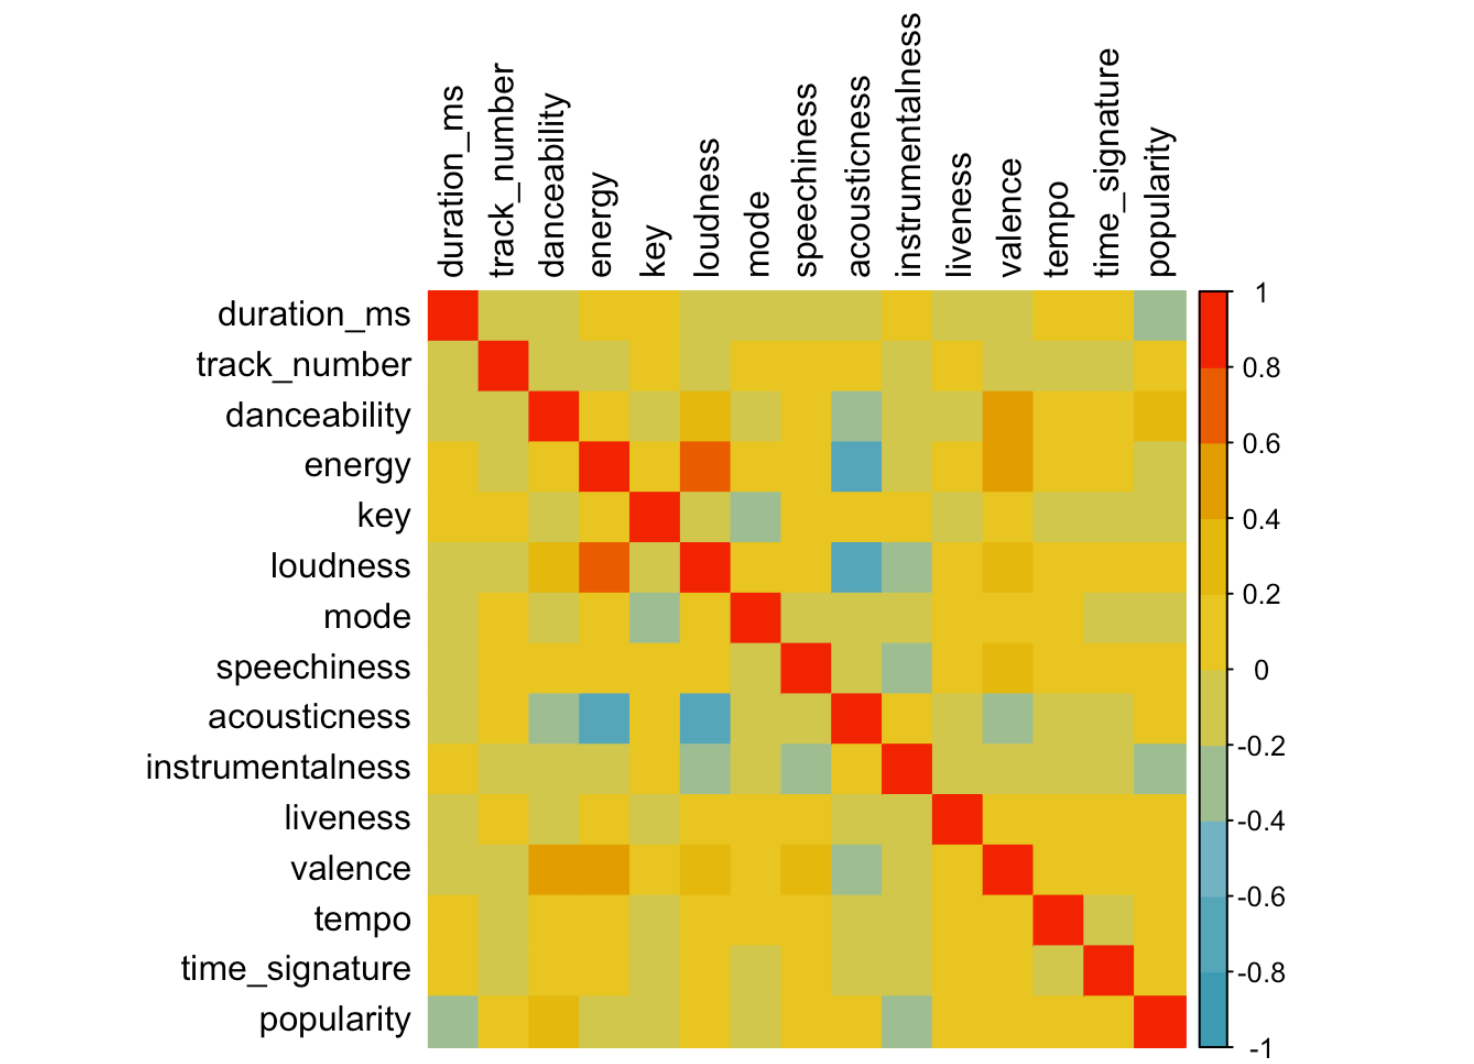
\includegraphics[width = \columnwidth]{spotify-images/multicollinear}}
\caption{Correlation plot for the Spotify API track features.}
\label{fig:corrplot}
\end{figure}

The variables that are highest correlated with another align at a darker red or darker blue square. Some of these variables seem to be correlated with one another, but they make sense. Loudness is correlated with energy because the loudness of a track is used to compute the energy of a song from the spotify dataset. From this, we would wager there is not much wrong here despite needing some interaction terms for the regression. 

The multiple regression involves most of these variables except for duration and track number. The signficant predictors for valence are danceability, energy, speechiness, acousticness, and instrumentalness.  Fig.~\ref{fig:regress} shows the regression results. Another significant factor is the intercept, which became significant after the addition of the interaction terms in the model. 

All of the significant predictors make sense, so we might expect a relationship between different songs/albums to be built on their valence as described by these significant features. 

\begin{figure}
\centerline{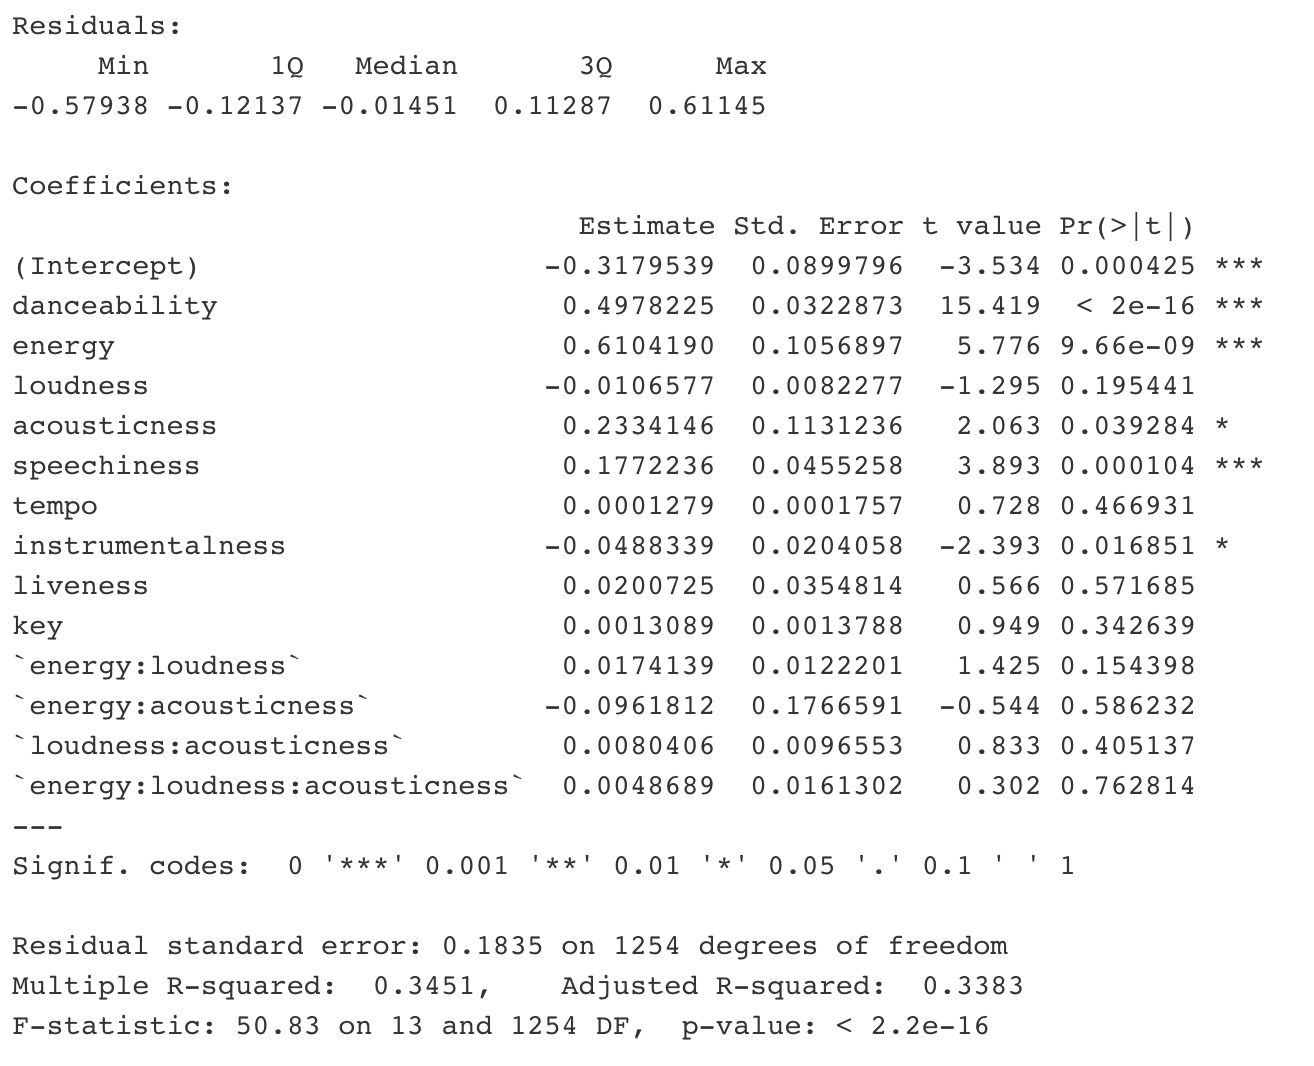
\includegraphics[width = \columnwidth]{spotify-images/regression}}
\caption{Summary of Regression Results}
\label{fig:regress}
\end{figure}

\subsection{Trends Over the 2010s}

To see how valence has changed over the decade, we will use a time series plot to visualize trends. These plots contain both an LOESS line and a regular linear model line. The linear model line is to establish the direction of trends while the LOESS line represents the local stability of that trend.   Fig.~\ref{fig:ts_album} shows a time series plot of all of the albums in the dataset and their respective average valence. 

\begin{figure}[htbp]
\centerline{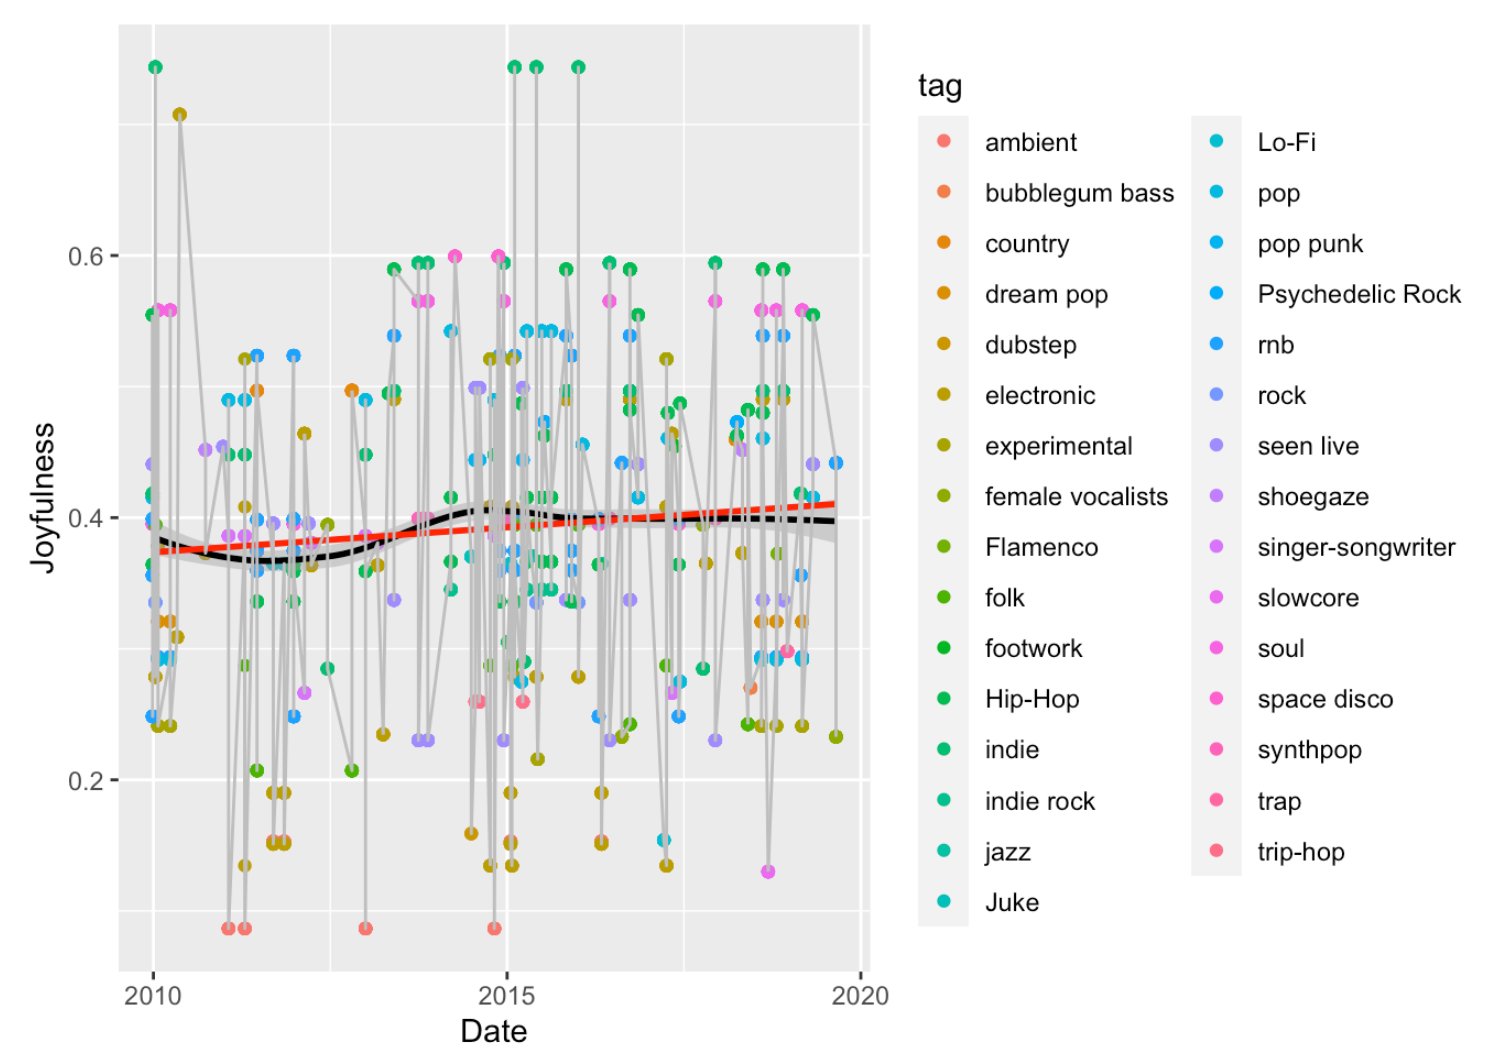
\includegraphics[width = \columnwidth]{spotify-images/joy_ts_album}}
\caption{Time Series plot of joyfulness in albums}
\label{fig:ts_album}
\end{figure}

Fig.~\ref{fig:ts_album} shows that that, over time, valence is increasing across the decade. The LOESS line shows that songs were temporarily much sadder in around late 2012. It looks like there are some positive outliers in hip hop being being the most positive albums of the bunch, while ambient music and electronic music tend to be the saddest. 

\begin{figure}[htbp]
\centerline{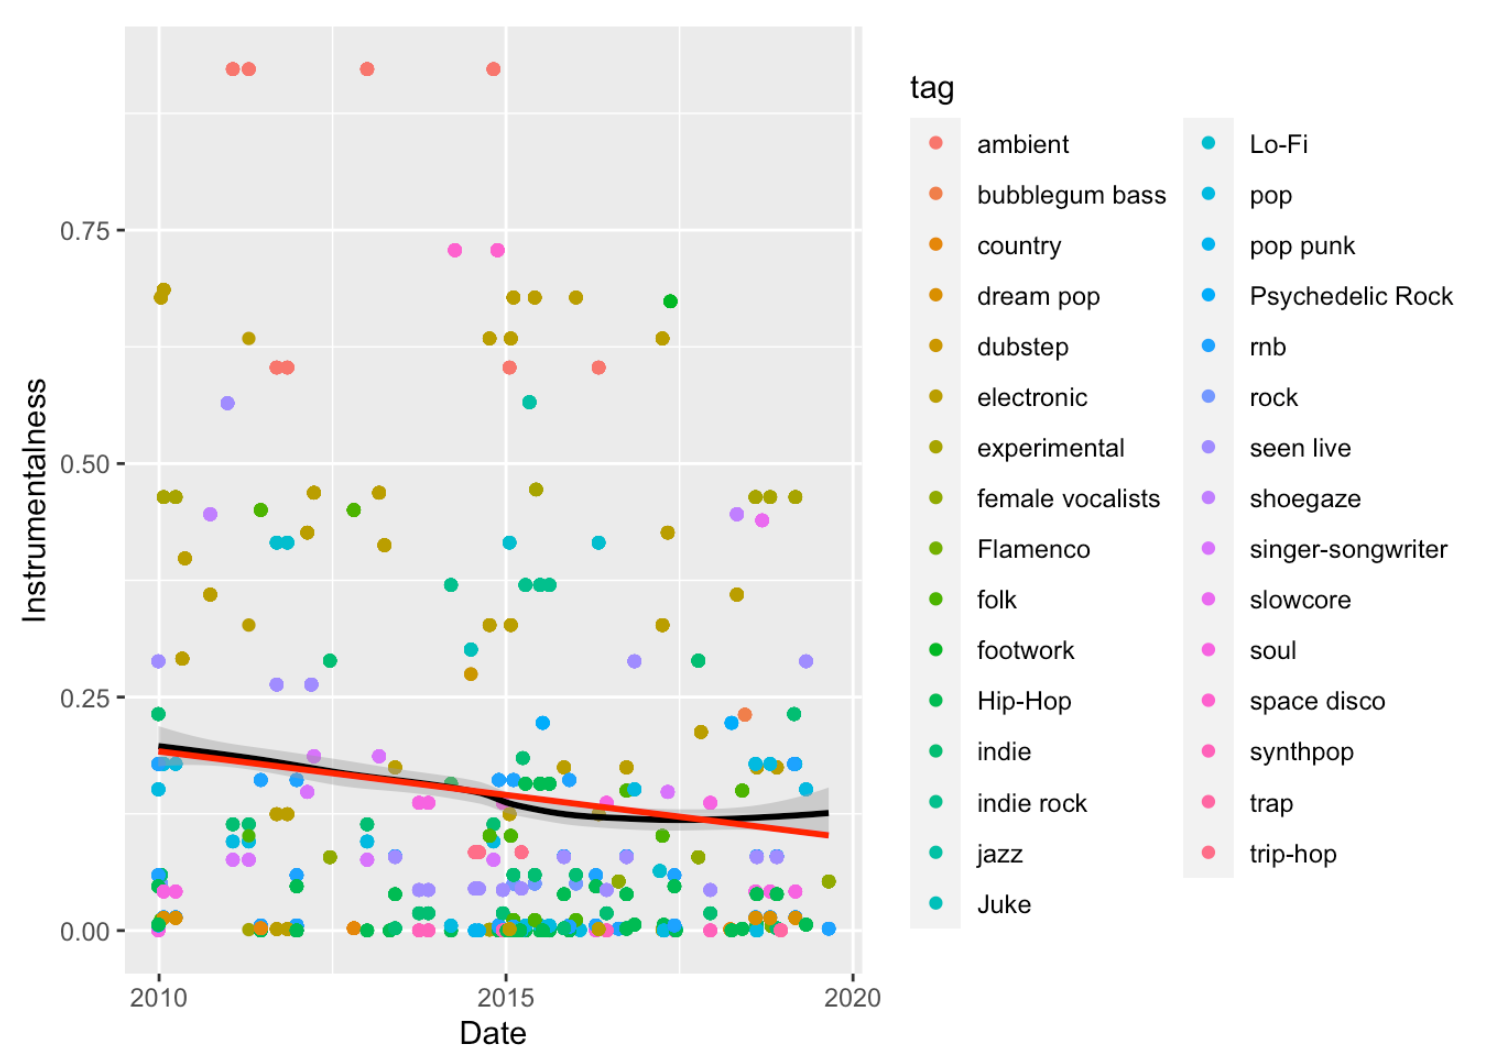
\includegraphics[width = \columnwidth]{spotify-images/vocal_ts_album}}
\caption{Time Series plot of vocality in albums}
\label{fig:ts_album_v}
\end{figure}

What about the vocality or "instrumentalness" of albums? It is sometimes said that music is saying less nowadays since electronic instrumentation and less lyrics have become more popular. Fig~\ref{fig:ts_album_v} shows this time series plot. 

It actually seems to be that there have been a higher amount of vocality in albums throughout the decade in general as well as increasing vocality toward the end of the decade. 

\subsection{Hierarchical Clustering}

With an analysis done on the data, we are ready to begin clustering the data. Using the methods defined, a hierarchical clustering algorithm with complete linkage is ran. Fig.~\ref{fig:circlize} shows the results plotted in a radial dendrogram.

\begin{figure}[htbp]
\centerline{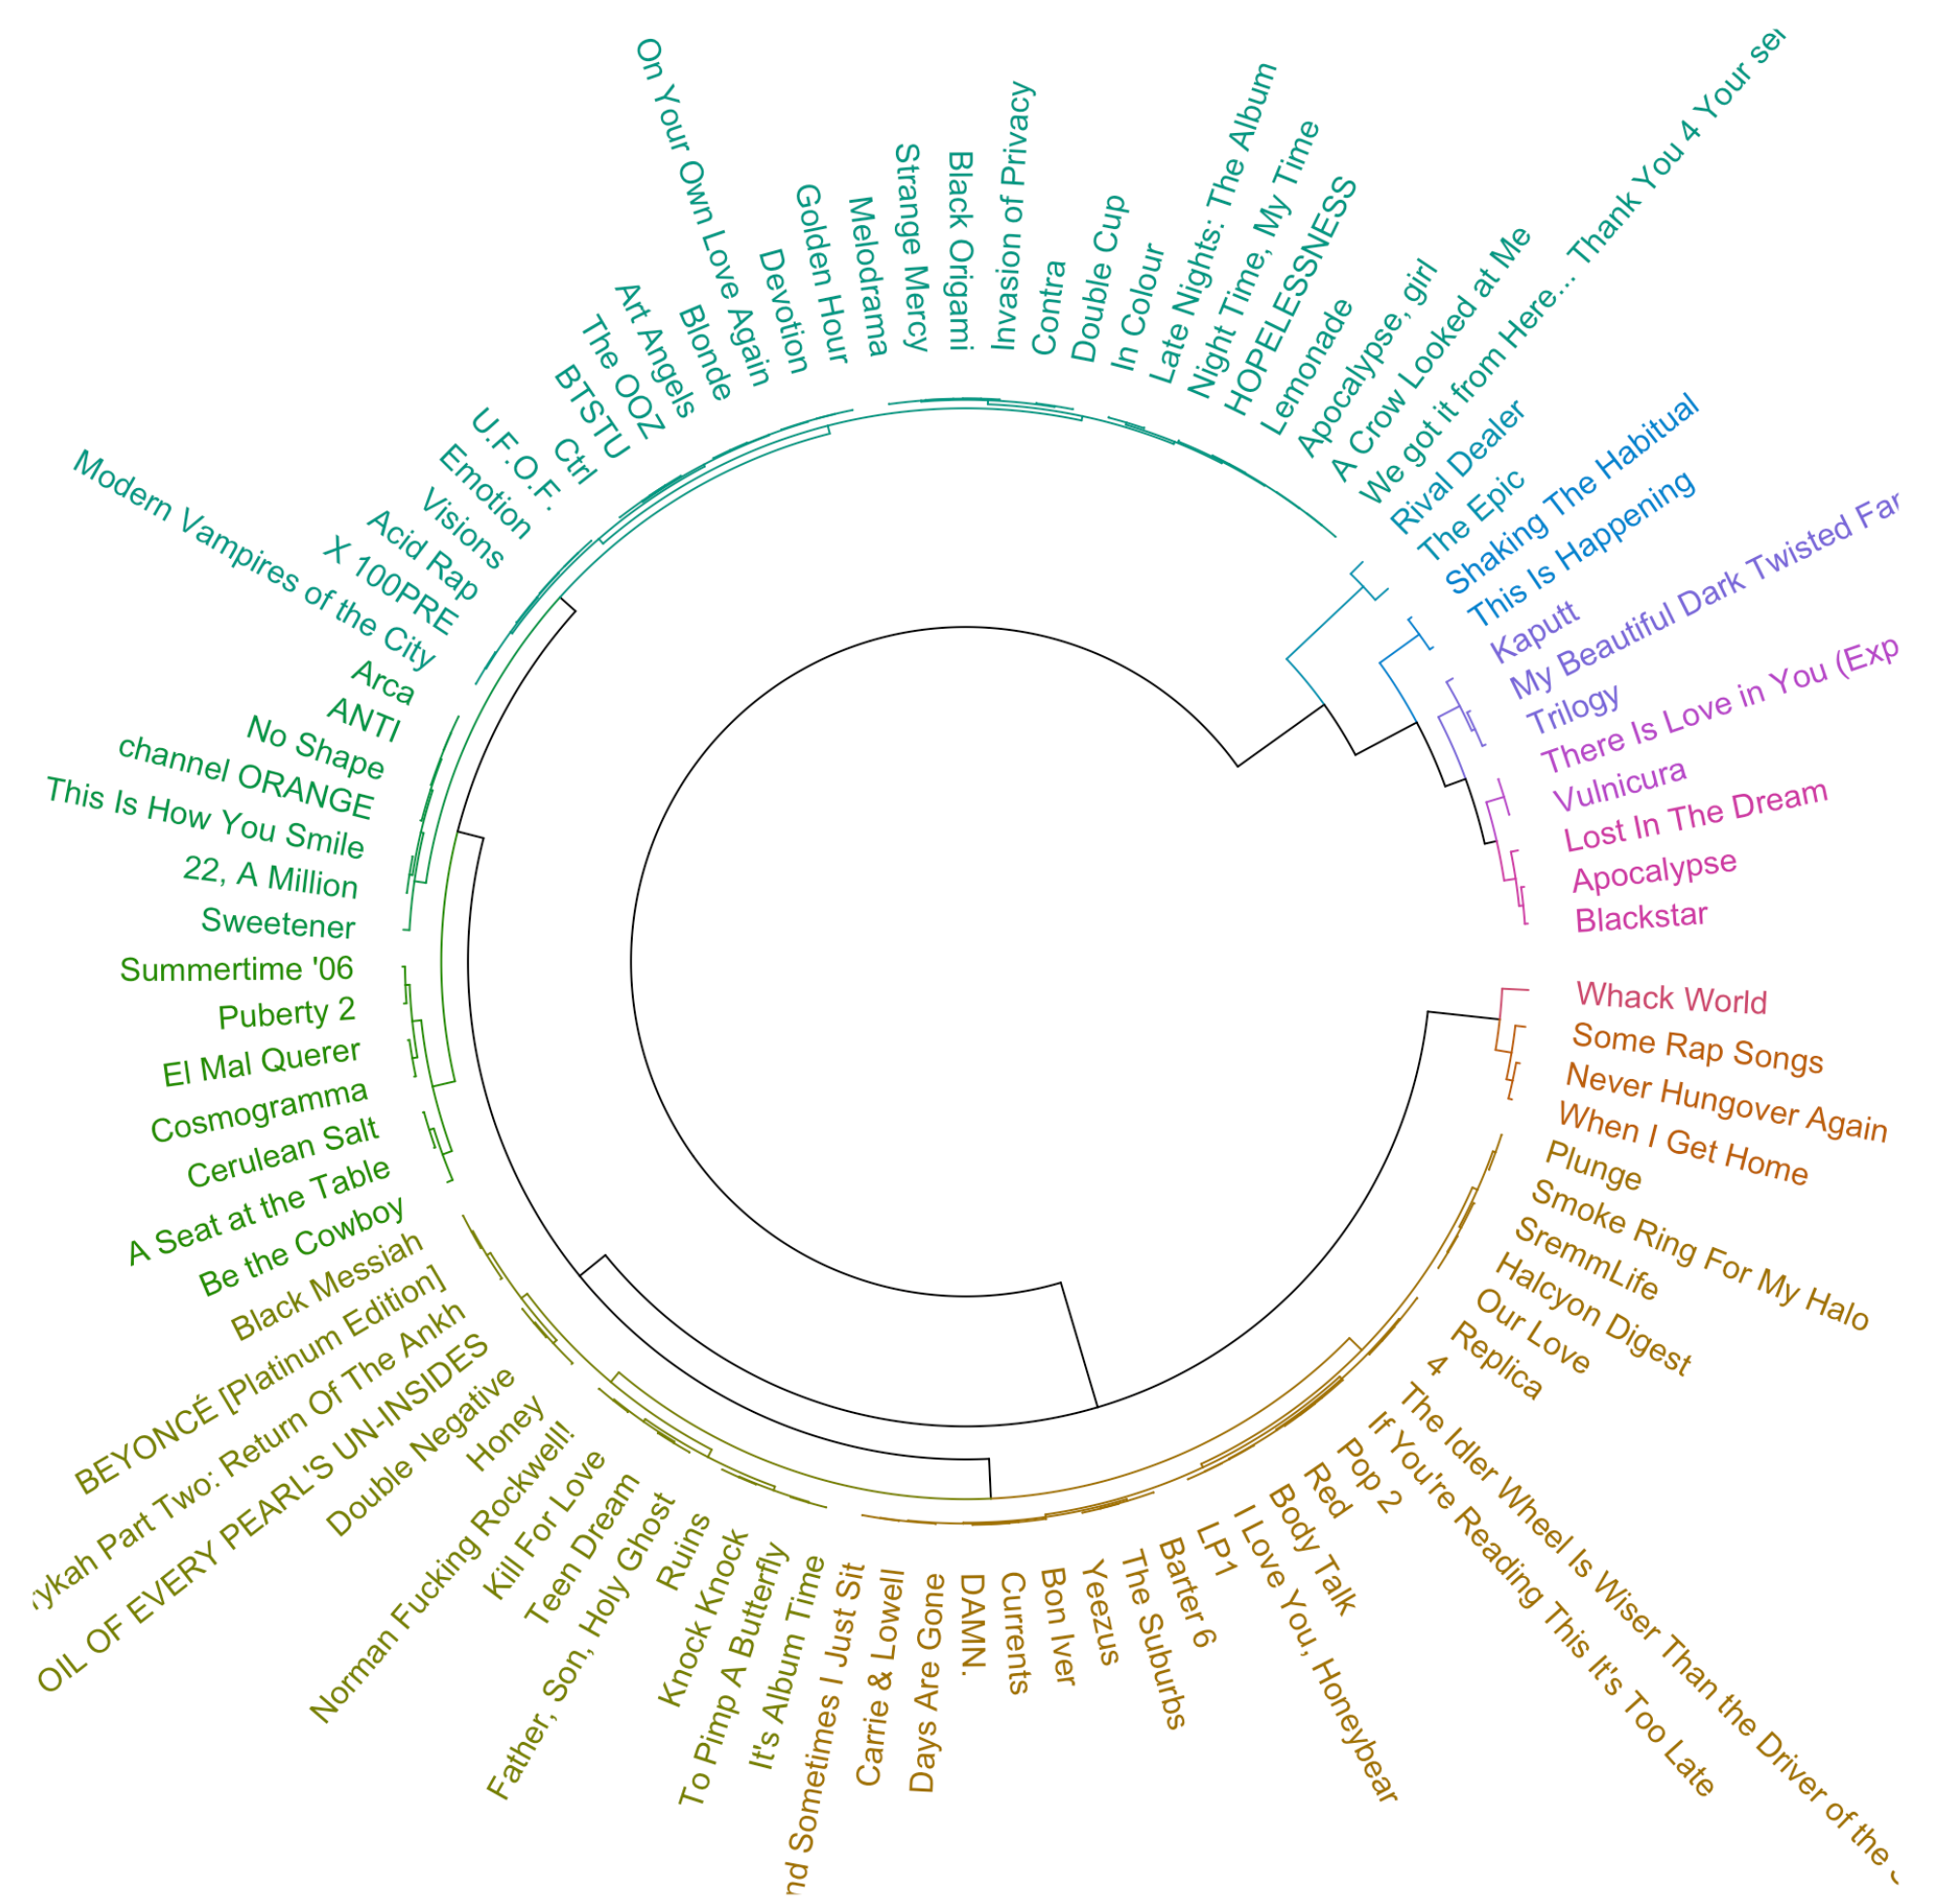
\includegraphics[width = \columnwidth]{spotify-images/circlize}}
\caption{Radial Dendrogram of albums}
\label{fig:circlize}
\end{figure}

For this figure, each of the larger clusters are colored together. Ideally, these would be colored by their genres for genre-genre comparisons. This however, could not be figured out in time for this work.

Despite this, some surprising features arise from the data. Generally speaking, the hip-hop music seems to be clustered into the brown section, RnB is generally in the green sections, and pop is in the green and dark yellow sections. This of course is not consistent for 100\% of the items in those sections, but it is a relative approximation based on eyesight. 

Albums like \textit{To Pimp a Butterfly} are linked with albums like \textit{Norman F* Rockwell} in the dark yellow section despite the fact that they seemed to be on opposite ends of the emotional spectrum in Fig.~\ref{fig:most-joyful}. Collections like this are likely due to other factors than just the valence comparison shown in Fig.~\ref{fig:most-joyful}. Considering the two albums, \textit{To Pimp a Butterfly} is a very soul/funk inspired album despite it being an album designated as "hip-hop". This might have resonated with some of the deeper, subdued sounds that are present on a subtle indie album like \textit{Norman F* Rockwell}. 

This is perhaps an indicator that this model really extracts the subtle features of the tracks and albums despite there being genre tags included. An approach like this should be great for a recommendation algorithm that not only needs to create recommendations based on the genres of music, but also the subtle, less describable feelings conveyed underneath the labels and tags. 

Another example that draws attention is the albums \textit{El mal Querer} and \textit{Cosmogramma}, the former being a flamenco-pop record while the latter being an electronic record. Both of these records likely carry some feature-driven relationship that could not be seen with a comparison of genres and genre archetypes. 

\section{Conclusion}

This investigation involved the clustering analysis of the spotify data compiled from the spotify API through an R wrapper. Developing a criterion for investigation, the data were visualized and compared to understand identifiable characteristics that a hierarchical clustering model might pick up. This included an analysis on the level of valence and instrumentalness conveyed across albums, an analysis of the collinearity of the parameters, and an analysis on the trends seen over the decade. 

We saw that Hip-hop generally had happier songs, songs with more lyrics tended to be happier, and that happiness in albums seemed to be increasing across the decade. We also demonstrated a linear regression to show which features were significant in estimating happiness, as well as seeing which features were highly correlated with each other to estimate pairwise interactions.

Finally, we ran a hierarchical clustering model that created groupings based on spotify's features that were both surprising and insightful. This technique could most likely be a valid way to develop a robust recommendation system to recommend other genres with similar "musical feelings" to keep users engaged and listening. 

There are some caveats with this method however. Unless Spotify releases exactly how each of the features are developed/calculated, there is no way of academically defining exactly what each feature means in a consistent context. This harms the clustering techniques since unrelated clusters can be created based on a feature space that was developed itself with the use of an algorithm. The algorithm is essentially a black-box to everyone other than spotify. 

Future works should be a development of this hierarchical clustering into categories of users based on data. Then perhaps compared with popularity metrics to see if the clusters correctly include the relevant albums that may improve listening time. 

\section*{Acknowledgment}

S. Sargolzaei, thanks for the help on defining and understanding the statistical background of this work. 

\begin{thebibliography}{00}
\bibitem{b1} Z. He, X. Xu, S. Deng, "Clustering Mixed Numeric and Categorical Data: A cluster Ensemble Approach". . 2005.
\bibitem{b2} J. van den Hoven, "Analysing Spotify Data", 3rd ed., VU University, August 2015.
\bibitem{b3 } G. James, D. Witten, T. Hastie, R. Tibshirani. An Introduction to Statistical Learning : with Applications in R. New York :Springer, 2013.
\bibitem{b4} Spotify API,  'https://developer.spotify.com/documentation/web-api/reference/tracks/get-audio-features/', Spotify.
\bibitem{b5} T. Charlie, spotifyr, ``https://www.rcharlie.com/spotifyr/'' 
\bibitem{b6} Iyanaga, S., \& Kawada, Y. (1980). Statistical Estimation and Statistical Hypothesis
Testing. (Vol. Appendix A, Table 23). Cambridge, MA: MIT Press.
\bibitem{b7} R. Tibshirani and T. Hastie. (1987). Local Likelihood estimation. J. Amer. Statist. Assn. 82, 558-567.
\bibitem{b8} NIST, "LOESS (aka LOWESS)", section 4.1.4.4, NIST/SEMATECH e-Handbook of Statistical Methods, (accessed 19 April 2020)
\bibitem{b9} R. Berman, 2018, "This is the music people listen to..." https://bigthink.com/robby-berman/how-americans-self-medicate-with-music. \textit{BigThink}. 
\end{thebibliography}


\end{document}
